%!TEX root = ./slopecd.tex

\section{Theory}\label{sec:theory}
%%%%%%%%%%%%%%%%%%%%%%%%%%%%%%%%%%%%
\subsection{Coordinate Descent for SLOPE}%
\label{sec:coordinate-updates}

\mathurin{Suggestion: \\
Proximal coordinate descent cannot be applied to \Cref{pb:slope} because it is not separable.
However, if the clusters $\mathcal{C}_1, \ldots, \mathcal{C}_m$ of the solution $\hat \beta$ were known together with its sign, then the values $c_1, \ldots, c_m$ taken by $\hat \beta$ on the clusters could be equivalently computed by solving :
\begin{problem}
\min_{x \in \bbR^m}
F \left(\sum_{i=1}^m \tilde{X}_i x_i \right)
+ \sum_{i=1}^m (\sum_{\lambda \in \lambda^{\mathcal{C}_i}} \lambda) x_i \enspace,
\end{problem}
where $\tilde{X}_{\mathcal{C}_i} = \sum_{j \in \mathcal{C}_i} X_j \sign (\hat \beta_j)$.
Hence, the idea of our algorithm is to intertwine steps that identify the clusters, and large coordinatewise steps on these clusters.
}
Based on this observation, we derive a coordinate descent algorithm for minimizing the SLOPE problem~\eqref{pb:slope} with respect to the coefficients of a single cluster at a time.
First observe that we can write \Cref{pb:slope} as \mathurin{To discuss:  we restrict to quadratic datafit? in the intro there's a generic df and our strategy would be adapted to it, it's just block coordinate descent with varying blocks}
\[
  \begin{aligned}
    P(\beta)
     & =  \frac{1}{2} \lVert y - X\beta\rVert_2^2 + J(\beta)                        \\
     & = \frac{1}{2} \lVert y - X_{\bar{\mathcal{C}_k}} \beta_{\bar{\mathcal{C}_k}}
    - \big(X_{\mathcal{C}_k} s_{\mathcal{C}_k}\big)c_k  \rVert_2^2
    + |c_k|\sum_{j \in {\mathcal{C}_k}} \lambda_{(j)^-}
    + \sum_{j \notin {\mathcal{C}_k}} |\beta_j|\lambda_{(j)^-}                      \\
     & = \frac{1}{2} \lVert \tilde r - \tilde x c_k \rVert_2^2
    + |c_k|\sum_{j \in {\mathcal{C}_k}} \lambda_{(j)^-}
    + \sum_{j \notin {\mathcal{C}_k}} |\beta_j|\lambda_{(j)^-}                      \\
  \end{aligned}
\]
with \( \tilde x_k = X_{\mathcal{C}_k} s_{\mathcal{C}_k}\) and
\(\tilde r_k = y - \tilde y_k = y - X_{\bar{\mathcal{C}}_k} \beta_{\bar{\mathcal{C}}_k} \in \bbR^n\).
\mm{do we need $\tilde y _k$ ?}
\mathurin{What is tricky here is that $\beta$ varies so the $C_k$ and $c_k$ vary too. THe notation $C_k(\beta)$ would be too heavy (most of all because $m$ also depends on $\beta$, but so I would avoid writing such computations that are confusing IMO - at least they confused me to be honest)}

\mathurin{I would just say we perform block coordinate descent update/directional updates in the direction of $(\sign \beta)_{\mathcal{C_i}}$
}
We propose a coordinate-wise update that minimizes \(P(\beta)\) with respect to the
clusters' corresponding coefficients one at a time, keeping the relative signs
of the coordinates within each cluster fixed but allowing all of the signs to
flip (simultaneously).

Letting \(\beta\) correspond to a fixed vector, note that
\(\beta_i = s_i c_{(j)^-}\), \(i \in \mathcal{C}_j\) for all
\(i\). Now let \(\tilde{\mathcal{C}}_i\)
correspond to the indices of the \(i\)th cluster for \(\beta\), that is,
\(|\beta_j| = c_i\) for all \(j \in \tilde{\mathcal{C}}_i\).
Next, we let
\begin{equation}
  \label{eq:coordinate-update-beta}
  \beta_i(z) =
  \begin{cases}
    s_k z   & \text{if } i \in \mathcal{C}_k, \\
    \beta_i & \text{otherwise.}
  \end{cases}
\end{equation}
\mathurin{maybe we can write $\beta + z \sign(\beta)_{\mathcal{C}_i}$, where $\sign$ is the sign vector, and restricting indices keeps the dimension (and puts 0 as value of excluded indices).}
This means that \(\beta(x)\) corresponds to a version of \(\beta\) with a
coordinate update for the \(k\)th cluster.

This corresponds to solving the following
one-dimensional problem:

\begin{equation}
  \label{eq:cluster-problem}
  \operatorname*{minimize}_{z \in \mathbb{R}} \left(P_k(z) = \frac{1}{2} \lVert \tilde r - \tilde x z \rVert_2^2 + J_k(z)\right)
\end{equation}
where
\[
  J_k(z) = |z| \sum_{j \in \mathcal{C}_k} \lambda_{(j)^-_z}
  + \sum_{j \notin \mathcal{C}_k} |\beta_j| \lambda_{(j)^-_z}
\]
is the \emph{partial sorted \(\ell_1\) norm} with respect to the \(k\)th cluster and
\mm{new notation; we could write $(j; \beta(z))$ or $(j; \beta + z d)$, $d$ being the direction}
where we write \(\lambda_{(j)^-_z}\) to indicate that the permutation operator \((j)^-_z\)
is defined through \(\beta(z)\).

The optimality condition for this problem is
\[
  P_k'(z; \delta) \geq 0,
\]
where \(P'_k(z; \delta)\) is the directional derivative of \(P_k\).
Note that we have
\[
  P_k'(z; \delta) = \delta\big(\tilde x^T \tilde x z - \tilde r^T \tilde x\big) + J'_k(z; \delta)
\]
since \(\lVert \tilde{r} - \tilde{x}z\rVert_2^2\) is differentiable.

\mathurin{One key aspect of such updates that for me deserves to be emphasized: the clusters will almost all remain the same: they can only change order, or two of them merge.}

Throughout the rest of this section section we will derive a minimizer
solution to \eqref{eq:cluster-problem}. To do so, we will introduce the
directional derivative for the sorted \(\ell_1\) norm with respect to the
coefficient of the \(k\)th cluster. First, however, let
\(C(z)\) be a function that returns the cluster corresponding to \(z\), that is
\[
  C(z) = \{j : |\beta(z)_j| = z\}.
\]
Next, let there be an \({\varepsilon_c} > 0\) such that
\begin{equation}
  \label{eq:epsilon-c}
  \big| c_i - c_j\big| > {\varepsilon_c} \quad \forall\, i \neq j
\end{equation}
for a strictly decreasing sequence \(c_1, c_2, ..., c_m\).

For a\({\varepsilon_c}\) and \(\delta \in \{-1, 1\}\)\mathurin{This can be hard to parse: $C$ implicitly depends on a vector that determines clusters. We can emphasize that  In all this section $\beta$ is fixed and we update only in the direction given by the sign of one cluster. Clusters $C_i$ and $c_i$ are fixed.}
we have
\begin{equation}
  \lim_{h \downarrow 0} C(z + h\delta) = C(z + {\varepsilon_c} \delta)
  \quad\text{and}\quad
  \lim_{h \downarrow 0} \lambda_{(i)^-_{z + h\delta}}
  = \lambda_{(i)^-_{z + {\varepsilon_c}\delta}}.
\end{equation}
In other words, the order permutation corresponding to \(\beta(z + h\delta)\)
depends only on \(\delta\) in the limit as \(h\) tends to~\(0\).
\begin{remark}
  As consequence of the definition of \(\varepsilon_c\), the order permutations
  for \(\beta(z)\) and \(\beta(z + {\varepsilon_c} \delta)\) differ only for a
  subset of the permutation vectors. The permutation for \(\beta(h\delta)\)
  corresponds to
  \[
    \begin{cases}
      \tilde{\mathcal{C}}_1, \dots, \tilde{\mathcal{C}}_{k-1}, \tilde{\mathcal{C}}_{k+1}, \dots, \tilde{\mathcal{C}}_m, C({\varepsilon_c}\delta)                                          & \text{if } c_m > 0 \text{ and } \delta \neq 0, \\
      \tilde{\mathcal{C}}_1, \dots, \tilde{\mathcal{C}}_{k-1}, \tilde{\mathcal{C}}_{k+1}, \dots, C({\varepsilon_c}\delta), \tilde{\mathcal{C}}_m                                          & \text{if } c_m = 0 \text{ and } \delta \neq 0, \\
      \tilde{\mathcal{C}}_1, \dots, \tilde{\mathcal{C}}_{k-1}, \tilde{\mathcal{C}}_{k+1}, \dots, \underbrace{\tilde{\mathcal{C}}_k \cup \tilde{\mathcal{C}}_m}_{C({\varepsilon_c}\delta)} & \text{if } c_m = 0 \text{ and } \delta = 0.    \\
    \end{cases}
  \]
  The permutation for \(\beta(z + {\varepsilon_c} \delta)\), \(z \neq 0\) corresponds to
  \[
    \begin{cases}
      \tilde{\mathcal{C}}_1, \dots, \tilde{\mathcal{C}}_{k-1}, \tilde{\mathcal{C}}_{k+1}, \dots, C(c_i + {\varepsilon_c}\delta), \tilde{\mathcal{C}}_i, \dots, \tilde{\mathcal{C}}_m                                          & \text{if } \delta = 1,  \\
      \tilde{\mathcal{C}}_1, \dots, \tilde{\mathcal{C}}_{k-1}, \tilde{\mathcal{C}}_{k+1}, \dots, \tilde{\mathcal{C}}_i, C(c_i + {\varepsilon_c}\delta), \dots, \tilde{\mathcal{C}}_m                                          & \text{if } \delta = -1, \\
      \tilde{\mathcal{C}}_1, \dots, \tilde{\mathcal{C}}_{k-1}, \tilde{\mathcal{C}}_{k+1}, \dots, \underbrace{\tilde{\mathcal{C}}_i \cup \tilde{\mathcal{C}}_k}_{C(c_i + {\varepsilon_c}\delta)}, \dots, \tilde{\mathcal{C}}_m & \text{if } \delta = 0.  \\
    \end{cases}
  \]
\end{remark}

We are now ready to state the directional derivative of \(J_k\).

\begin{theorem}\label{thm:sl1-directional-derivative}
  The directional derivative of \(J_k\) in the direction \(\delta\) is
  \[
    J'_k(z, \delta) =
    \begin{cases}
      \smashoperator[r]{\sum_{j \in C({\varepsilon_c} \delta)}} \lambda_{(j)^-_{{\varepsilon_c}\delta}}                    & \text{if } z = 0,         \\
      \sign(z)\delta\smashoperator{\sum_{j \in C(z + {\varepsilon_c} \delta)}} \lambda_{(j)^-_{z + {\varepsilon_c}\delta}} & \text{if } |z| = c_i > 0, \\
      \sign(z)\delta\smashoperator{\sum_{j \in C(z)}} \lambda_{(j)^-_{z}}                                                  & \text{otherwise,}
    \end{cases}
  \]
  with \({\varepsilon_c}\) defined as in \eqref{eq:epsilon-c}.
\end{theorem}
\begin{proof}
  The directional derivative of \(J_k\) in the direction \(\delta\), with
  \(|\delta| = 1\), is defined as
  \begin{align}
    J_k'(z; \delta)
    = & \lim_{h \downarrow 0} \frac{J_k(z + h \delta) - J_k(z)}{h} \nonumber \\
    = &
    \lim_{h \downarrow 0} \frac{1}{h}
    \left(
      |z + h \delta| \smashoperator{\sum_{j \in C(z + h \delta)}} \lambda_{(j)^-_{z + h \delta}}
      + \smashoperator{\sum_{j \notin C(z + h\delta)}} |\beta_j| \lambda_{(j)^-_{z + h \delta}}
      - |z| \smashoperator{\sum_{j \in C(z)}} \lambda_{(j)^-_z}
      - \smashoperator{\sum_{j \notin C(z)}} |\beta_j| \lambda_{(j)^-_z}
    \right) \nonumber                                                        \\
    = & \lim_{h \downarrow 0}
    \frac{1}{h}
    \left(
      |z + h \delta| \smashoperator{\sum_{j \in C(z + {\varepsilon_c}\delta)}} \lambda_{(j)^-_{z + {\varepsilon_c}\delta}}
      + \smashoperator{\sum_{j \notin C(z + {\varepsilon_c}\delta)}} |\beta_j| \lambda_{(j)^-_{z + {\varepsilon_c}\delta}}
      - |z| \smashoperator{\sum_{j \in C(z)}} \lambda_{(j)^-_{z}}
      - \smashoperator{\sum_{j \notin C(z)}} |\beta_j| \lambda_{(j)^-_{z}}
    \right)
    \label{eq:directional-derivative-sl1}
  \end{align}
  We have the following cases to consider: \(|z| = c_i\) for \(i \neq k\),
  \(|z| = 0\), and \(z \notin \{0, c_i\}\) for \(i \neq k\).

  Turning first to the case when \(|z| = c_i\) for \(i \neq k\), note that we have,
  as a result of the definition of
  \({\varepsilon_c}\), the following identities:
  \begin{align*}
    C(c_i + {\varepsilon_c}\delta)          & \subseteq C(c_i),                                                                                                                     \\
    \tilde{\mathcal{C}}_i                   & = \widebar{C(c_i + {\varepsilon_c} \delta)} \cap C(c_i),                                                                              \\
    C(c_i)                                  & = \tilde{C}_i \cup \big(C(c_i + {\varepsilon_c}\delta) \cap C(c_i)\big) = \tilde{\mathcal{C}}_i \cup C(c_i + {\varepsilon_c} \delta), \\
    \widebar{C(z + {\varepsilon_c} \delta)} & = \widebar{C(c_i)} \cup \tilde{\mathcal{C}}_i.
  \end{align*}
  Using this, we can rewrite \eqref{eq:directional-derivative-sl1} as
  \begin{equation*}
    \label{eq:directional-derivative-simplified}
    J'_k(z; \delta)
    = \lim_{h \downarrow 0} \frac{1}{h}
    \left(
      \splitfrac{
      |z + h\delta|\smashoperator{\sum_{j \in C(z + {\varepsilon_c}\delta)}} \lambda_{(j)^-_{z + {\varepsilon_c}\delta}}
      + |c_i|\smashoperator{\sum_{j \in \tilde{C}_i}} \lambda_{(j)^-_{z + {\varepsilon_c}\delta}}
      + \smashoperator{\sum_{j \in \widebar{C(z)}}} |\beta_j|\lambda_{(j)^-_{z + {\varepsilon_c}\delta}}
      }{%
      - |z| \smashoperator{\sum_{j \in \tilde{\mathcal{C}}_i}} \lambda_{(j)^-_{z}}
      - |c_i| \smashoperator{\sum_{j \in C(z + {\varepsilon_c}\delta)}} \lambda_{(j)^-_{z}}
      - \smashoperator{\sum_{j \in \widebar{C(z)}}} |\beta_j| \lambda_{(j)^-_{z}}
      }
    \right).
  \end{equation*}
  Next, observe that \(\lambda_{(j)^-_{z + {\varepsilon_c}\delta}} =
  \lambda_{(j)^-_{z}}\) for all \(j \in \widebar{C(z)}\) and consequently
  \[
    \smashoperator{\sum_{j \in \widebar{C(z)}}} |\beta_j|\lambda_{(j)^-_{z + {\varepsilon_c}\delta}} =
    \smashoperator{\sum_{j \in \widebar{C(z)}}} |\beta_j|\lambda_{(j)^-_{z}}.
  \]
  Moreover, note that, since \(z = \pm c_i\), there exists a permutation corresponding to
  \(\lambda_{(j)^-_{z}}\) such that
  \[
    |z|\smashoperator{\sum_{j \in \tilde{C}_i}} \lambda_{(j)^-_{z + {\varepsilon_c}\delta}}
    = |c_i| \smashoperator{\sum_{j \in \tilde{C}_i}} \lambda_{(j)^-_{z}}
  \]
  and consequently
  \begin{equation}
    \label{eq:directional-derivative-simplified-again}
    J'_k(z; \delta)
    = \lim_{h \downarrow 0} \frac{1}{h}
    \left(
      |z + h\delta|\smashoperator{\sum_{j \in C(z + {\varepsilon_c}\delta)}} \lambda_{(j)^-_{z + {\varepsilon_c}\delta}}
      - |c_i| \smashoperator{\sum_{j \in C(z + {\varepsilon_c}\delta)}} \lambda_{(j)^-_{z}}.
    \right).
  \end{equation}
  Now, since \(c_i + h \delta > 0\) and \(-c_i + h \delta < 0\) in the limit as
  \(h\) goes to \(0\) for \(c_i \neq 0\), we have
  \[
    \lim_{h\downarrow 0} |-c_i + h \delta|
    = \lim_{h\downarrow 0}\big( |c_i| -h \delta\big)
    \quad\text{and}\quad
    \lim_{h\downarrow 0} |c_i + h \delta|
    = \lim_{h\downarrow 0}(|c_i| + h \delta)
  \]
  which means that
  \begin{align*}
    J'_k(z; \delta)
     & = \lim_{h \downarrow 0} \frac{1}{h}
    \left(
      \big(|z| + \sign(z)h\delta\big)\smashoperator{\sum_{j \in C(z + {\varepsilon_c}\delta)}} \lambda_{(j)^-_{z + {\varepsilon_c}\delta}}
      - |c_i| \smashoperator{\sum_{j \in C(z + {\varepsilon_c}\delta)}} \lambda_{(j)^-_{z}}.
    \right)                                                                                                                  \\
     & = \lim_{h \downarrow 0} \frac{1}{h}
    \sign(z)h\delta\smashoperator{\sum_{j \in C(z + {\varepsilon_c}\delta)}} \lambda_{(j)^-_{z + {\varepsilon_c}\delta}}     \\
     & = \sign(z)\delta\smashoperator{\sum_{j \in C(z + {\varepsilon_c}\delta)}} \lambda_{(j)^-_{z + {\varepsilon_c}\delta}} \\
  \end{align*}

  In the case when \(z = c_i = 0\), that is, we have \(\beta_k = 0\) for some \(k\),
  then
  \eqref{eq:directional-derivative-simplified-again} is simply
  \begin{equation*}
    \label{eq:directional-derivative-zerocase}
    J'_k(0; \delta)
    = \lim_{h \downarrow 0} \frac{1}{h}
    |h\delta|\smashoperator{\sum_{j \in C({\varepsilon_c}\delta)}} \lambda_{(j)^-_{{\varepsilon_c}\delta}}
    = \smashoperator{\sum_{j \in C({\varepsilon_c}\delta)}} \lambda_{(j)^-_{{\varepsilon_c}\delta}}
  \end{equation*}
  since \(|\delta| = 1\) by definition,

  Proceeding, now, with the case when \(z = 0 \neq c_i\), \(i \neq k\),
  we see that \eqref{eq:directional-derivative-sl1} reduces to
  \begin{equation*}
    J_k'(0; \delta) = \lim_{h \downarrow 0}
    \frac{1}{h}
    \left(
      |h \delta| \smashoperator{\sum_{j \in C({\varepsilon_c}\delta)}} \lambda_{(j)^-_{{\varepsilon_c}\delta}}
      + \smashoperator{\sum_{j \notin C({\varepsilon_c}\delta)}} |\beta_j| \lambda_{(j)^-_{{\varepsilon_c}\delta}}
      - \smashoperator{\sum_{j \notin C(0)}} |\beta_j| \lambda_{(j)^-_{0}}
    \right).
  \end{equation*}
  In this case, we have \(C(0) = C({\varepsilon_c}\delta)\) since \(c_m \neq 0\), and therefore
  \[
    \smashoperator{\sum_{j \notin C({\varepsilon_c}\delta)}} |\beta_j| \lambda_{(j)^-_{{\varepsilon_c}\delta}}
    = \smashoperator{\sum_{j \notin C(0)}} |\beta_j| \lambda_{(j)^-_{0}},
  \]
  which means that
  \begin{equation*}
    J_k'(0; \delta) = \lim_{h \downarrow 0}
    \frac{1}{h}
    |h \delta| \smashoperator{\sum_{j \in C({\varepsilon_c}\delta)}} \lambda_{(j)^-_{{\varepsilon_c}\delta}}
    = |\delta|\smashoperator{\sum_{j \in C({\varepsilon_c}\delta)}} \lambda_{(j)^-_{{\varepsilon_c}\delta}}
    = \smashoperator{\sum_{j \in C(0)}} \lambda_{(j)^-_{0}}.
  \end{equation*}

  Finally, note that \(J_k\) is differentiable in every other case, that is,
  \(|z| \notin \{0, c_i\}\) for \(i \neq k\) and, since since \(C(z +
  {\varepsilon_c}\delta) = C(z)\), has the directional derivative
  \[
    J_k'(z; \delta) = \delta \sign(z) \smashoperator{\sum_{j \in C(z)}} \lambda_{(j)^-_{z}}.
  \]
\end{proof}

We are now ready to present the SLOPE thresholding operator.

\begin{theorem}[The SLOPE Thresholding Operator]
  \[
    T_k(\gamma, \omega; c, \lambda) =
    \begin{cases}
      0                                                                                                                                                   & \text{if } |\gamma| \leq \smashoperator{\sum_{j \in C({\varepsilon_c})}} \lambda_{(j)^-_{\varepsilon_c}},                                                                                                                                                        \\
      \sign(\gamma)c_i                                                                                                                                    & \text{if } \omega c_i + \smashoperator{\sum_{j \in C(c_i - {\varepsilon_c})}} \lambda_{(j)^-_{c_i - {\varepsilon_c}}} \leq |\gamma| \leq \omega c_i + \smashoperator{\sum_{j \in C(c_i + {\varepsilon_c})}} \lambda_{(j)^-_{c_i + {\varepsilon_c}}},             \\
      \frac{\sign(\gamma)}{\omega} \bigg( |\gamma| - \smashoperator{\sum_{j \in C(c_i + {\varepsilon_c})}} \lambda_{(j)^-_{c_i + {\varepsilon_c}}} \bigg) & \text{if } \omega c_i + \smashoperator{\sum_{j \in C(c_i + {\varepsilon_c})}} \lambda_{(j)^-_{c_i + {\varepsilon_c}}} < |\gamma| < \omega c_{i - 1} + \smashoperator{\sum_{j \in C(c_{i - 1} - {\varepsilon_c})}} \lambda_{(j)^-_{c_{i - 1} - {\varepsilon_c}}}, \\
      \frac{\sign(\gamma)}{\omega} \bigg( |\gamma| - \smashoperator{\sum_{j \in C(c_1 + {\varepsilon_c})}} \lambda_{(j)^-_{c_1 + {\varepsilon_c}}} \bigg) & \text{if } |\gamma| \geq \omega c_1 + \smashoperator{\sum_{j \in C(c_1 + {\varepsilon_c})}} \lambda_{(j)^-_{c_1 + {\varepsilon_c}}}.
    \end{cases}
  \]
  with \({\varepsilon_c}\) defined as in \eqref{eq:epsilon-c} and let
  \(\gamma = \tilde{r}^Tx\), \(\omega = \tilde{x}^T\tilde{x}\). Then
  \(T(\gamma, \omega; c; \lambda) \in \argmin_{z \in \mathbb{R}} J_k(z)\).
\end{theorem}
\begin{proof}
  \jw{Help the reader what you want todo. Also structure it clearer so it can be followed easier. Right now you start with $z$ conditions then move to $\gamma$ conditions.}
  Recall that \(J_k(z) : \mathbb{R} \mapsto \mathbb{R}\) is a convex,
  continuous piecewise-differentiable function with kinks whenever \(|z| = c_i\) or \(z = 0\). Let \(\gamma =
  \tilde{r}^T\tilde{x}\) and \(\omega = \tilde{x}^T\tilde{x}\) and note that
  the optimality criterion for \eqref{eq:cluster-problem} is
  \[
    \delta(\omega z - \gamma) + J'_k(z; \delta) \geq 0, \quad
    \forall \delta \in \{-1, 1\},
  \]
  which is equivalent to
  \begin{equation}
    \label{eq:optimality-inequality}
    \omega z - J'_k(z; -1) \leq \gamma \leq \omega z + J_k'(z; 1).
  \end{equation}

  Now observe that \(z = 0\) is a solution to \(\argmin_{z \in \mathbb{R}}
  J_k(z)\) if and only if
  \begin{equation}
    \label{eq:case-zero}
    - J'_k(0; -1) \leq \gamma \leq J_k'(0; 1) \implies
    | \gamma | \leq \smashoperator{\sum_{j \in C({\varepsilon_c})}}\lambda_{(j)^-_{{\varepsilon_c}}}
  \end{equation}
  since \(C({\varepsilon_c}) = C(-{\varepsilon_c})\) and
  \(\lambda_{(j)^-_{-{\varepsilon_c}}} = \lambda_{(j)^-_{{\varepsilon_c}}}\).

  Next, \(z = c_i \neq 0\), \(i \neq k\) is a solution if and only if
  \begin{equation}
    \label{eq:case-cluster}
    \omega c_i + \smashoperator{\sum_{j \in C(c_i - {\varepsilon_c})}} \lambda_{(j)^-_{c_i - {\varepsilon_c}}}
    \leq |\gamma| \leq
    \omega c_i + \smashoperator{\sum_{j \in C(c_i + {\varepsilon_c})}} \lambda_{(j)^-_{c_i + {\varepsilon_c}}}
  \end{equation}
  since \(C(c_i + {\varepsilon_c}) = C(-c_i - {\varepsilon_c})\) and
  \(C(-c_i + {\varepsilon_c}) = C(c_i - {\varepsilon_c})\).

  If neither \eqref{eq:case-zero} nor \eqref{eq:case-cluster} hold, then it must either
  be the case that
  \begin{equation}
    \label{eq:differentiable-inequality}
    \omega c_i + \smashoperator{\sum_{j \in C(c_i + {\varepsilon_c})}} \lambda_{(j)^-_{c_i + {\varepsilon_c}}}
    < |\gamma| <
    \omega c_{i - 1} + \smashoperator{\sum_{j \in C(c_{i - 1} - {\varepsilon_c})}} \lambda_{(j)^-_{c_{i - 1} - {\varepsilon_c}}},
  \end{equation}
  for some \(i > 1\), or that
  \[
    |\gamma| > \omega c_1 + \smashoperator{\sum_{j \in C(c_1 + {\varepsilon_c})}} \lambda_{(j)^-_{c_1 + {\varepsilon_c}}}.
  \]
  In the first case, note that
  \[
    \smashoperator{\sum_{j \in C(c_i + {\varepsilon_c})}} \lambda_{(j)^-_{c_i + {\varepsilon_c}}}
    =
    \smashoperator[r]{\sum_{j \in C(c_{i-1} - {\varepsilon_c})}} \lambda_{(j)^-_{c_{i-1} - {\varepsilon_c}}}
  \]
  and therefore \eqref{eq:differentiable-inequality} is equivalent to
  \[
    c_i < \frac{1}{\omega} \bigg( |\gamma| - \smashoperator{\sum_{j \in C(c_i + {\varepsilon_c})}} \lambda_{(j)^-_{c_i + {\varepsilon_c}}} \bigg) < c_{i -1}.
  \]
  Let
  \[
    z^* = \frac{\sign(\gamma)}{\omega} \bigg( |\gamma| - \smashoperator{\sum_{j \in C(c_i + {\varepsilon_c})}} \lambda_{(j)^-_{c_i + {\varepsilon_c}}} \bigg)
  \]
  Note that \(|z^*| \in (c_i, c_{i-1})\) and
  % for a \(z \in (c_i, c_{i-1})\), observe that
  \[
    \frac{1}{\omega} \bigg( |\gamma| - \smashoperator{\sum_{j \in C(c_i + {\varepsilon_c})}} \lambda_{(j)^-_{c_i + {\varepsilon_c}}} \bigg)
    =
    \frac{1}{\omega} \bigg( |\gamma| - \smashoperator{\sum_{j \in C(z^*)}} \lambda_{(j)^-_{z^*}} \bigg).
  \]
  Furthermore, since \(P_k\) is differentiable in \((c_i, c_{i-1})\), we have
  % which is exactly the optimum for \(P_k(z)\) since it is
  % differentiable for \(|z| \in (c_i, c_{i -1})\) and \(|z| > c_1\) and has a
  % unique minimizer
  \[
    \frac{\partial}{\partial z} P_k(z) \Big|_{z = z^*}
    = \omega z^* - \gamma + \sign(z^*) \smashoperator{\sum_{j \in C(z^*)}} \lambda_{(j)^-_{z^*}} = 0.
  \]
  The case \(|z| > c_1\) follow analogously.
\end{proof}

\jl{Consider adding a remark showing that our operator generalizes the soft thresholding operator.}

In \cref{fig:slope-thresholding}, we visualize the SLOPE thresholding operator.

\begin{figure}[htbp]
  \centering
  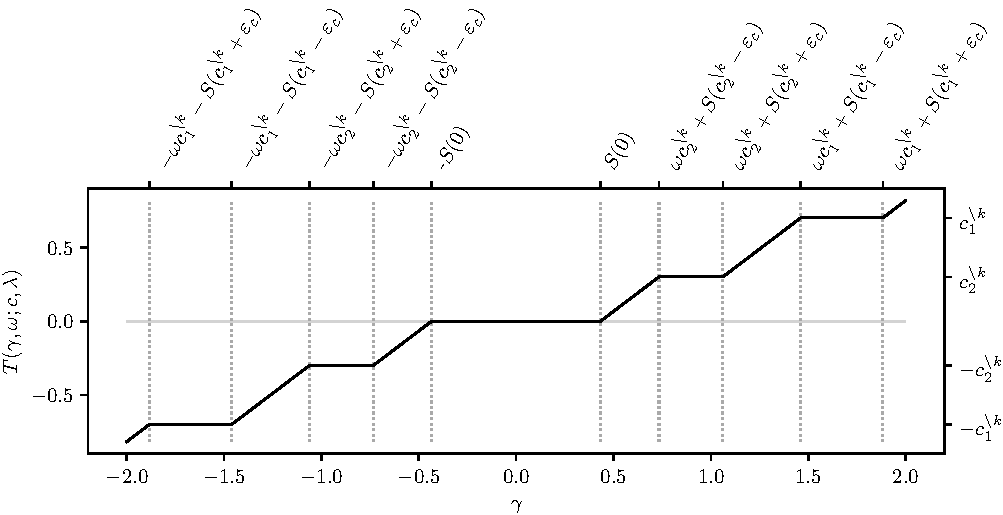
\includegraphics[]{slope-thresholding.pdf}
  \caption{The result of the SLOPE thresholding update.}
  \label{fig:slope-thresholding}
\end{figure}

\subsubsection{Naive Updates}

As in \textcite{friedman2010}, we can improve the efficiency of updates by observing that
\begin{equation*}
  \begin{aligned}
    \tilde r_k & = y - \tilde y_k                                                                       \\
               & = y - X_{\bar{\mathcal{C}}_k}\beta_{\bar{\mathcal{C}}_k} - \tilde x c_k + \tilde x c_k \\
               & = r + \tilde x c_k
  \end{aligned}
\end{equation*}
and therefore that
\begin{equation}
  \label{eq:naive-update}
  \tilde x_k^T (y - \tilde y_k) = \tilde x_k^T r + \tilde x_k^T \tilde x_k c_k.
\end{equation}

\subsubsection{Caching Reductions}

Observe that \(\tilde x_k\) only changes between subsequent coordinate updates provided that the members of the cluster \(k\) change, for instance if two clusters are merged, a predictor leaves a cluster, or the signs flip (through an update of \(\alpha_k\)).
As a result, it is possible to obtain computational gains by caching \(\tilde x_k\) and \(\tilde x_k^T \tilde x_k\) for each cluster (except the zero cluster, which we do not consider in our coordinate descent step).
When there is no change in the clusters, there is no need to recompute these quantities.
And even when there are changes, we can still reduce the costs involved since \(\tilde x_k\) can be updated in place.
If a large cluster is joined by few new predictors, then the cost of updating may be much lower than recomputing the quantities for the entire cluster.
Also note that, for single-member clusters we only need to store \(\tilde x_k^T \tilde x_k\) since \(\tilde x_k\) is just a column in \(X\) times the corresponding sign.

Letting \(\tilde x_k^\text{old}\) correspond to the value of \(\tilde x_k\) before the update, we note that \(\tilde x_k \gets \tilde x_k^\text{old} + x_j \sign(\beta_j)\) for each \(j \in \mathcal{C}_k^\text{new} \setminus \mathcal{C}_k^\text{old}\) and \(\tilde x_k \gets \tilde x_k^\text{old} - x_j \sign(\beta_j)\) for each \(j \in \mathcal{C}_k^\text{old} \setminus \mathcal{C}_k^\text{new}\).
If only the signs flip, we simply have to also flip the signs in \(\tilde x_k\).

\subsubsection{Covariance Updates}

Notice that we can rewrite the first term in \eqref{eq:naive-update} as
\begin{equation}
  \begin{aligned}
    \tilde x_k^T r & = \tilde x_k^T y - \sum_{j : \beta_j \neq 0} \tilde x_k^T x_j \beta_j                                                                    \\
                   & = \tilde x_k^T y - \sum_{j : c_j \neq 0} \tilde x_k^T \tilde x_j c_j                                                                     \\
                   & = s_{\mathcal{C}_k}^T X_{\mathcal{C}_k}^T y - \sum_{j : \beta_j \neq 0} s_{\mathcal{C}_k}^T X_{\mathcal{C}_k}^T x_j \beta_j              \\
                   & = s_{\mathcal{C}_k}^T \left(X^T y\right)_{\mathcal{C}_k} - \sum_{j : \beta_j \neq 0} s_{\mathcal{C}_k}^T X_{\mathcal{C}_k}^T x_j \beta_j \\
                   & = \sum_{j \in \mathcal{C}_k}\left( s_j x_j^Ty - \sum_{t : \beta_t \neq 0} s_j x_j^T x_t \beta_t \right)
  \end{aligned}
\end{equation}
As in \textcite{friedman2010}, this formulation can be used to achieve so-called \emph{covariance updates}.
We compute \(X^T y\) once at the start.
Then, each time a new predictor becomes non-zero, we compute its inner product with all other predictors, caching these products.

\subsection{Hybrid proximal coordinate descent strategy}

We propose an iterative solver that alternates between proximal gradient step and proximal coordinate descent.
Since the regularization term for SLOPE is not separable, applying PCD does not guarantee convergence (show example where CD gets stuck).
However, \cite{dupuis2021} showed that once the clusters are known, the subdifferential of $J$ can be written as the cartesian product of the subdifferential of $J$ restricted to the clusters.
Hence, if one knew the clusters, PCD updates could be applied on each cluster.

The notion of clusters for SLOPE extends the notion of sparsity coming from the LASSO.
Identification of the sparsity pattern throughout the iterative algorithm have largely been studied.
Talk about Partly Smooth functions, related Manifold and that support transpose to cluster for SLOPE regularization. DO the maths.

Then identification of this underlying structure occurs when applying PGD.
Hence the idea to alternate, PGD and PCD step to take advantage of the speed of PCD and ensure convergence via the identification of the right structure with PGD steps.

\begin{algorithm}[tb]
  \SetKwInOut{Init}{init}
  \SetKwInOut{Input}{input}
  \caption{%
    Hybrid coordinate descent and proximal gradient descent algorithm
    for SLOPE\label{alg:hybrid}}
  \Input{
    \(X \in \mathbb{R}^{n\times p}, y\in \mathbb{R}^n, \beta\in \mathbb{R}^p, \lambda \in \{\mathbb{R}^p : \lambda_1 \geq \lambda_2 \geq \cdots > 0\}\), \(m \in \mathbb{N}\)}

  \Init{\(t \gets 0\), \(\beta \gets 0\), \(L \gets \lVert X \rVert_2^2\)}

  \Repeat{convergence}{
  \(t \gets t + 1\)

  \If{\(t \bmod m = 0\)}{

  \(\beta \leftarrow \operatorname{prox}_{J / L}(\beta - \frac{1}{L}\nabla f(\beta))\) \label{alg:hybrid-istastep}

  % \(C_1, \hdots, C_m \leftarrow \mathtt{get\_clusters}(\beta)\)
  }
  \Else{
    \(k \gets 0\)

    \While{\(k \leq \lvert \mathcal{C} \rvert\)}{
      \(k \gets k + 1\)

      \(s \leftarrow \mathrm{sign}(\beta_{\mathcal{C}_k})\)

      \If{\(s \neq 0\)}{
        % \(L_k \gets (X_{:, \mathcal{C}_k}s)^\top  X_{:, \mathcal{C}_k}s\)


        % \(\tilde{\beta} \gets T(|\beta_{\mathcal{C}_k}| - \frac{1}{L_k} \nabla_{\mathcal{C}_k}f(\beta)^\top s, \frac{\lambda}{L_k})\)

        % \(\beta_{\mathcal{C}_k} \leftarrow \tilde{\beta} s\)
        \(\tilde x_k \gets X_{\mathcal{C}_k}s\)

        \(\tilde y_k \gets X_{\widebar{\mathcal{C}}_k}\beta_{\widebar{\mathcal{C}}_k}\)

        \(\tilde r_k \gets y - \tilde y_k\)

        \(
        \beta_{\mathcal{C}_k} \gets
        s T \left(
        \frac{\tilde r^T_k \tilde x_k, }{ \tilde x_k^T \tilde x_k},
        \frac{\lambda}{ \tilde x_k^T \tilde x_k},
        k,
        \tilde \beta,
        \mathcal{C}
        \right)
        \)
        \Comment{\(\mathcal{C}\) is updated at this step.}


      }

    }
  }

  }
  \Return{\(\beta\)}
\end{algorithm}

\begin{theorem}
  Iterates of \cref{alg:hybrid} converge towards \(\beta^*\).
\end{theorem}
\begin{proof}
  First note that convergence properties of proximal gradient descent on convex
  problems such as SLOPE are well-established
  \parencite{beck2009,daubechies2004}, which certifies that updates via
  \cref{alg:hybrid-istastep} make progress towards \(\beta^*\).

  Next note that the objectives of \eqref{pb:slope} and
  \eqref{eq:subproblem} are equal and that \eqref{eq:subproblem} can be seen
  viewed as a version of \eqref{pb:slope} with added linear constraints
  that is also convex. And, finally, because the coordinate updates of
  \cref{alg:hybrid} minimize the sub-problem, we in the worst case make no
  progress and therefore have guaranteed converge rate no less than \(1/m\)
  of that of proximal gradient descent.
\end{proof}

